\documentclass[conference]{IEEEtran}

% ---------------------------------------------------------------------------
% Offline RL literature review, official IEEE conference template (conference_101719: IEEEtran, conference mode).
% Compiles with pdflatex (run twice). No external .bib file is needed: the
% reference list is embedded below in IEEE reference style, numbered in order
% of first citation.
% ---------------------------------------------------------------------------

% "nocompress" writes citation lists out in full, [1], [2], [3], as the IEEE
% Reference Style Guide requires (no en-dash ranges).
\usepackage[nocompress]{cite}
\usepackage{amsmath,amssymb,amsfonts}
\usepackage{array}
\usepackage{booktabs}
\usepackage{tabularx}
\usepackage{graphicx}
\usepackage{tikz}
\usetikzlibrary{positioning,arrows.meta}
\usepackage{textcomp}
\usepackage{xcolor}
\usepackage{url}
\usepackage{flushend} % balances the two columns on the last page
\usepackage[hidelinks]{hyperref}

\newcolumntype{L}{>{\raggedright\arraybackslash}X}
\newcolumntype{P}[1]{>{\raggedright\arraybackslash}p{#1}}

\hyphenation{off-line re-in-force-ment con-ser-va-tism}

\begin{document}

\title{Offline Reinforcement Learning: A Literature Review of Conservatism, Calibrated Uncertainty, and the Credibility of Evidence}

\author{\IEEEauthorblockN{David Bayha}
\IEEEauthorblockA{\textit{ITSC 8110} \\
\textit{University of North Carolina at Charlotte}\\
Charlotte, NC, USA}}

\maketitle

\begin{abstract}
Offline reinforcement learning (RL) aims to learn decision-making policies from a fixed dataset of previously collected experience, with no further interaction with the environment. The promise matters most where trial and error is costly or unsafe, but it has proved hard to realize: value estimates for actions that the dataset does not contain cannot be corrected, and policy optimization selects for the resulting errors. This paper reviews the literature on that problem. It analyzes 18 research papers published between 2019 and 2026 and three earlier surveys, places them within the foundational literature, and organizes the discussion around three themes: 1) conservatism toward actions that the data do not support; 2) calibrated and adaptive conservatism, in which uncertainty estimates decide how much caution to apply and where; and 3) the credibility of the evidence on which claims of progress rest. The review finds that the main algorithm families apply one remedy at different points of the learning pipeline and control it with a single hyperparameter per dataset, that calibration methods offer guarantees which cover less than the quantities that drive learning, and that a substantial share of reported progress is attributable to implementation choices and to tuning with online interaction. Strengths and limitations of the literature are assessed, and opportunities for future research are identified.
\end{abstract}

\begin{IEEEkeywords}
Batch reinforcement learning, calibration, conformal prediction, conservatism, distribution shift, offline reinforcement learning, pessimism, uncertainty quantification.
\end{IEEEkeywords}

% ===========================================================================
\section{Introduction}
% ===========================================================================
Reinforcement learning (RL) trains an agent to make sequential decisions by trial and error. In many of the domains where automated decision making would be most valuable, such as robotics, healthcare, and recommendation, trial and error is expensive or unsafe, while large logs of past decisions already exist \cite{levine2020tutorial,dulacarnold2021challenges}. Offline RL, historically called batch RL \cite{lange2012batch}, addresses this setting. The learner receives a fixed dataset collected by some behavior policy and must produce a better policy without any further interaction with the environment.

The research problem is that algorithms which succeed with interaction fail without it. Off-policy methods learn a value function by bootstrapping: the training target for one state-action pair depends on the estimated value of the action that the learned policy would take next. In the offline setting that next action may not appear anywhere in the dataset, so its estimated value is an unverified extrapolation. Because the policy is trained to prefer actions with high estimated value, it is drawn toward exactly those extrapolations whose errors are optimistic \cite{fujimoto2019bcq,kumar2019bear}. An online agent would try the action and observe its mistake. An offline learner never does, and the error propagates through subsequent updates.

A clinical example shows what is at stake. A policy for sepsis treatment was learned entirely from past intensive-care records \cite{komorowski2018clinician}. When its recommendations were later inspected case by case, it was found, for one group of stable patients, to prefer a treatment that only 6 patients in the data had received over the usual treatment given to 161 \cite{ji2021trajectory}. Six cases cannot establish that a treatment is better, yet the learned values ranked it best, and the recommendation could not responsibly be tested on patients. This review is organized around the question that such cases raise: how can an offline learner calibrate its caution to how well the data support each action, and how can a proposed answer be validated without the interaction that the setting rules out?

The question is significant for three reasons. First, a reliable answer would let RL reuse logged data in the way that supervised learning reuses labeled datasets \cite{levine2020tutorial}. Second, every known remedy trades safety against improvement: a learner held too close to the data cannot improve on it, and one allowed too far from the data exploits its own errors. Third, the credibility of the field depends on it, because a method intended for settings without interaction offers less than it appears to if its hyperparameters must be chosen with interaction \cite{paine2020hyperparameter,kurenkov2022budget}.

This review analyzes 18 research papers in depth. Three early works diagnosed the problem and proposed the first remedies: batch-constrained Q-learning (BCQ) \cite{fujimoto2019bcq}, bootstrapping error accumulation reduction (BEAR) \cite{kumar2019bear}, and behavior value estimation with ranking regularization (BRr) \cite{gulcehre2020brr}. Four define the main families of value-based offline RL: conservative Q-learning (CQL) \cite{kumar2020cql}, TD3 with behavior cloning (TD3+BC) \cite{fujimoto2021td3bc}, implicit Q-learning (IQL) \cite{kostrikov2022iql}, and the revisited behavior-regularized actor-critic (ReBRAC) \cite{tarasov2023rebrac}. A-Crab, an actor-critic regularized by average Bellman error \cite{zhu2023acrab}, represents the supporting theory, and the Unifloral study \cite{jackson2025unifloral} represents evaluation methodology. The uncertainty weighted actor-critic (UWAC) \cite{wu2021uwac} and the ensemble-diversified actor-critic (EDAC) \cite{an2021edac} derive conservatism from estimates of uncertainty, and quantile Q-learning (QQL) \cite{gao2026qql} and UNIQ \cite{upadhyay2026uniq} adapt it per state. BFN-RL \cite{killingberg2026bfn} is a generative planner that has no critic. Four further works calibrate value estimates or prediction intervals: conformal policy evaluation \cite{gan2025conformal}, Bellman calibration \cite{vanderlaan2026bellman}, conformal prediction as Bayesian quadrature (BQ-CP) \cite{snell2025bqcp}, and weighted Bayesian conformal prediction (WBCP) \cite{lou2026wbcp}. The review also examines three earlier surveys \cite{levine2020tutorial,he2023survey,prudencio2024survey} and reads all 21 works against the foundational literature on which they build.

The remainder of the paper is organized as follows. Section~\ref{sec:background} gives the necessary background. Section~\ref{sec:surveys} compares this review with the earlier surveys. Section~\ref{sec:organization} introduces the three themes and compares the 18 research papers along them. Sections~\ref{sec:theme1}, \ref{sec:theme2}, and~\ref{sec:theme3} treat the themes in turn. Section~\ref{sec:discussion} discusses strengths, limitations, and opportunities for future research, and Section~\ref{sec:conclusion} concludes.

% ===========================================================================
\section{Background}
\label{sec:background}
% ===========================================================================
\subsection{Problem Setting}
An RL problem is modeled as a Markov decision process with states $s \in \mathcal{S}$, actions $a \in \mathcal{A}$, transition dynamics $P(s' \mid s,a)$, reward function $r(s,a)$, and discount factor $\gamma \in [0,1)$. A policy $\pi(a \mid s)$ is judged by its expected discounted return
\begin{equation}
J(\pi) = \mathbb{E}_{\pi}\!\left[\sum_{t=0}^{\infty} \gamma^{t}\, r(s_t,a_t)\right].
\label{eq:return}
\end{equation}
where the expectation is over trajectories generated by following $\pi$. In the offline setting the learner is given a static dataset $\mathcal{D} = \{(s_i,a_i,r_i,s'_i)\}_{i=1}^{N}$ generated by an unknown behavior policy $\pi_\beta$ and must return a policy with high $J(\pi)$ using $\mathcal{D}$ alone \cite{levine2020tutorial}.

\subsection{Why Naive Offline Learning Fails}
Actor-critic methods fit an action-value function $Q$ by regressing it onto a bootstrapped target,
\begin{align}
y(r,s') &= r + \gamma\, \mathbb{E}_{a' \sim \pi(\cdot \mid s')}\big[\bar{Q}(s',a')\big], \label{eq:target}\\
\mathcal{L}(Q) &= \mathbb{E}_{(s,a,r,s') \sim \mathcal{D}}\Big[\big(Q(s,a) - y(r,s')\big)^{2}\Big], \label{eq:bellman}
\end{align}
where $\bar{Q}$ is a slowly updated copy of $Q$, and they improve the policy toward actions with high $Q$. The state-action pairs $(s,a)$ in \eqref{eq:bellman} are drawn from the data, but the action $a'$ in the target \eqref{eq:target} is chosen by the learned policy. When $\pi$ differs from $\pi_\beta$, the critic is evaluated at out-of-distribution (OOD) actions on which it was never trained. Fujimoto et al. \cite{fujimoto2019bcq} named the resulting inaccuracy \emph{extrapolation error} and showed that standard off-policy algorithms can fail to learn from fixed data because of it. Kumar et al. \cite{kumar2019bear} traced the instability to bootstrapping from OOD actions, whose errors accumulate through repeated backups. The mismatch between the state-action distribution of the dataset and the distribution induced by the learned policy is called \emph{distribution shift} \cite{levine2020tutorial}. Methods that deliberately bias learning against actions that the data do not support are called \emph{conservative} or \emph{pessimistic}; the two terms are used interchangeably in this review.

\subsection{Calibration and Conformal Prediction}
Two statistical ideas recur in the more recent works. A predictor $\hat{f}$ is \emph{calibrated} when its outputs match what is observed on average among the cases that receive the same prediction, that is, when $\mathbb{E}[y \mid \hat{f}(x) = v] = v$ for every value $v$. \emph{Conformal prediction} converts prediction errors measured on held-out data into prediction intervals with a finite-sample guarantee \cite{angelopoulos2023conformal}. In its simplest (split) form, the errors $e_i = |y_i - \hat{f}(x_i)|$ are computed on $n$ calibration pairs, $\hat{q}$ is set to their $\lceil (n+1)(1-\delta) \rceil / n$ empirical quantile for a chosen miscoverage level $\delta$, and the interval
\begin{equation}
C(x) = \big[\hat{f}(x) - \hat{q},\; \hat{f}(x) + \hat{q}\big]
\label{eq:conformal}
\end{equation}
is reported. If the calibration and test pairs are exchangeable, then $\Pr\{y \in C(x)\} \geq 1 - \delta$ for a new pair $(x,y)$, whatever the form of the data distribution. Two features of this guarantee matter below. It is marginal, holding on average over test points rather than for each $x$, and the interval in \eqref{eq:conformal} has the same width everywhere unless the errors are rescaled. Weighted variants extend the guarantee to covariate shift, in which test inputs are distributed differently from calibration inputs, by weighting each calibration error by the likelihood ratio between the two input distributions \cite{tibshirani2019covariate}. Offline RL strains both conditions: transitions within a trajectory are dependent, and the learned policy moves the distribution away from the data.

The term \emph{coverage} is used in this sense for prediction intervals. It is distinct from \emph{data coverage}, the extent to which a dataset contains the state-action pairs that a policy of interest would visit.

\subsection{Benchmarks and Reporting Conventions}
Most empirical results discussed below use D4RL \cite{fu2020d4rl}, a suite of simulated tasks that includes locomotion, maze navigation, dexterous manipulation, and kitchen tasks, with datasets that range from random behavior to expert demonstrations and mixtures of the two. Scores are normalized as
\begin{equation}
\text{score} = 100 \times \frac{R - R_{\mathrm{random}}}{R_{\mathrm{expert}} - R_{\mathrm{random}}},
\label{eq:score}
\end{equation}
where $R$ is the average return of the evaluated policy and $R_{\mathrm{random}}$ and $R_{\mathrm{expert}}$ are the returns of a random and an expert reference policy, so that 0 corresponds to random and 100 to expert performance. Papers commonly report sums or averages of normalized scores over groups of datasets. All scores quoted in this review follow that convention and are taken from the cited works.

% ===========================================================================
\section{Relation to Existing Surveys}
\label{sec:surveys}
% ===========================================================================
Three surveys address the same research question and were analyzed for this review (Table~\ref{tab:surveys}).

Levine et al. \cite{levine2020tutorial} wrote the tutorial that framed the field. It organizes the early methods by algorithmic principle (importance sampling, approximate dynamic programming with policy constraints, uncertainty penalties, or conservative critics, and model-based methods) under one notation and one diagnosis, namely distribution shift. Its findings anticipate two of the themes below. It judges that policy constraints must be tight, which caps improvement, and that uncertainty-based methods are principled but that calibrated uncertainty for deep value functions is hard to obtain; how to adjust pessimism to the data is left as an open problem. The tutorial stops in mid-2020, before TD3+BC, IQL, and ReBRAC, and it does not treat offline hyperparameter selection directly.

He \cite{he2023survey} gives a short primer on offline model-based RL that profiles seven methods by how each builds conservatism into a learned model of the environment. Its central observation is that a policy optimized inside a learned model drifts toward regions where the model is wrong but appears rewarding, and that the reward penalties used to prevent this \cite{kidambi2020morel,yu2020mopo} depend on uncertainty estimates that the survey regards as error-prone. It contains no benchmark results and no comparison table.

Prudencio et al. \cite{prudencio2024survey} provide the broad, structured update: a taxonomy that describes each algorithm as a class plus optional loss terms, a review of benchmarks and of off-policy evaluation (estimating the value of a policy from data collected by another), and a list of open problems led by reliable off-policy evaluation and hyperparameter tuning. Its coverage ends in early 2022, its treatment of uncertainty is confined to one line of ensemble work, and it names the dynamic adjustment of conservatism as an open problem without developing it.

This review differs from the three surveys in organization, coverage, and emphasis. It is organized by themes that cut across method families rather than by type of method. It covers work from 2023 to 2026 that none of them includes, including ReBRAC, A-Crab, budget-aware evaluation, and the adaptive and calibration-based methods. Finally, it takes as its second and third themes two matters that the surveys identify but leave open: conservatism that adapts to the data on the basis of calibrated uncertainty, and the reliability of the evidence used to compare methods. In exchange, its coverage is narrower, and like all three surveys it is a narrative review of expert-selected works rather than a systematic review with a reported search protocol.

\begin{table*}[!t]
\caption{Comparison With Existing Surveys}
\label{tab:surveys}
\centering
\footnotesize
\renewcommand{\arraystretch}{1.2}
\begin{tabularx}{\textwidth}{@{}P{0.13\textwidth}P{0.17\textwidth}LP{0.09\textwidth}L@{}}
\toprule
Review & Scope & Organizing principle & Coverage ends & Limits relevant to this review \\
\midrule
Levine et al. \cite{levine2020tutorial} & Offline RL as a whole & Algorithmic principle: importance sampling, dynamic programming, model-based methods & Mid-2020 & Predates TD3+BC, IQL, and ReBRAC; uncertainty-based methods treated briefly; offline hyperparameter selection not treated \\
He \cite{he2023survey} & Offline model-based RL & Profiles of seven methods & Early 2023 & No benchmark results or comparison table; model-free methods appear only as contrast \\
Prudencio et al. \cite{prudencio2024survey} & Deep offline RL, single agent & Taxonomy of algorithm classes and loss terms, with a benchmark review & Early 2022 & Dynamic adjustment of conservatism named but not developed; one line of uncertainty work; later methods absent \\
Present work & 18 research papers and three surveys & Three themes that cut across method families & 2026 & Narrative selection without a search protocol; narrower coverage; no new experiments \\
\bottomrule
\end{tabularx}
\end{table*}

% ===========================================================================
\section{Organization of the Review}
\label{sec:organization}
% ===========================================================================
Each of the 18 research papers was analyzed with a common set of questions covering its research question, contributions, method, results, validation, limitations, and ethical implications, and each survey with a parallel set covering its scope, method, findings, and limitations. Every work was then reduced to its three most central themes, and these were grouped into the three themes that organize the remainder of the paper.

\emph{Theme 1, conservatism toward unsupported actions} (Section~\ref{sec:theme1}), covers distribution shift, the tradeoff between conservatism and improvement, and behavior regularization. It is central to 12 of the 21 works, including all three surveys, and is the technical core of the field: every offline learner must decide how far to trust values that its data cannot verify.

\emph{Theme 2, calibrated and adaptive conservatism} (Section~\ref{sec:theme2}), covers uncertainty quantification and calibration, conservatism that varies per state or per sample, and conformal guarantees. It also spans 12 works and contains the single most prevalent topic, uncertainty quantification, which is central to 11. The theme responds to the finding of the surveys that existing uncertainty estimates are unreliable or hard to calibrate.

\emph{Theme 3, credibility of evidence} (Section~\ref{sec:theme3}), covers hidden implementation details and hyperparameter sensitivity, evaluation rigor, tuning with online interaction, minimalism, and the gap between theory and practice. It is the broadest theme, touching 11 works, and it matters because scores that depend on engineering choices and online tuning overstate what a user who is truly offline can expect.

The themes are linked, as Fig.~\ref{fig:themes} shows. Theme 1 creates the need for conservatism, Theme 2 concerns how much to apply and where, and Theme 3 determines whether a claimed answer to either can be trusted.

\begin{figure}[!t]
\centering
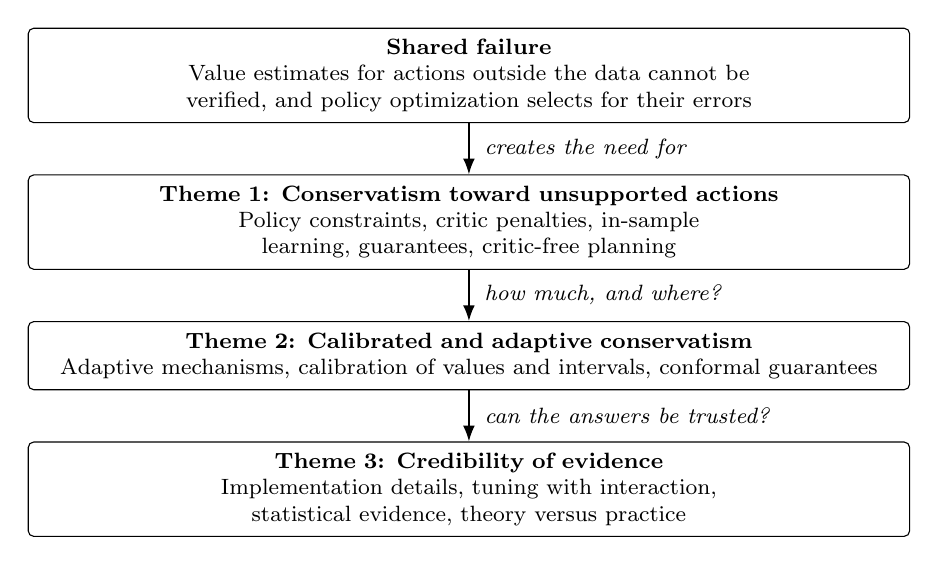
\begin{tikzpicture}[
  box/.style={draw, rounded corners=2pt, align=center, text width=0.9\columnwidth, inner sep=4pt, font=\footnotesize, execute at begin node={\hyphenpenalty=10000 \exhyphenpenalty=10000 }},
  lab/.style={font=\footnotesize\itshape, right=2pt},
  arr/.style={-{Latex[length=2mm]}, semithick}]
\node[box] (p) {\textbf{Shared failure}\\ Value estimates for actions outside the data cannot be verified, and policy optimization selects for their errors};
\node[box, below=6.5mm of p] (t1) {\textbf{Theme 1: Conservatism toward unsupported actions}\\ Policy constraints, critic penalties, in-sample learning, guarantees, critic-free planning};
\node[box, below=6.5mm of t1] (t2) {\textbf{Theme 2: Calibrated and adaptive conservatism}\\ Adaptive mechanisms, calibration of values and intervals, conformal guarantees};
\node[box, below=6.5mm of t2] (t3) {\textbf{Theme 3: Credibility of evidence}\\ Implementation details, tuning with interaction, statistical evidence, theory versus practice};
\draw[arr] (p) -- node[lab] {creates the need for} (t1);
\draw[arr] (t1) -- node[lab] {how much, and where?} (t2);
\draw[arr] (t2) -- node[lab] {can the answers be trusted?} (t3);
\end{tikzpicture}
\caption{Organization of the review. Each theme takes up the question left open by the one before it.}
\label{fig:themes}
\end{figure} Table~\ref{tab:comparison} compares the 18 research papers along the three themes.

\begin{table*}[!t]
\caption{Comparison of the 18 Research Papers Along the Three Themes}
\label{tab:comparison}
\centering
\footnotesize
\renewcommand{\arraystretch}{1.15}
\begin{tabularx}{\textwidth}{@{}P{0.105\textwidth}P{0.095\textwidth}LLL@{}}
\toprule
Work & Approach & Theme 1: conservatism toward unsupported actions & Theme 2: calibrated and adaptive conservatism & Theme 3: credibility of evidence \\
\midrule
BCQ \cite{fujimoto2019bcq} & Policy constraint & Generative model proposes actions near the data; a bounded perturbation limits departure from them & Hand-set perturbation bound, the same in every state & Guarantees cover tabular, deterministic problems; results shown only as learning curves \\
BEAR \cite{kumar2019bear} & Policy constraint & Policy held to the support of the data rather than to its distribution & One hand-set threshold for all states & Results shown only as learning curves; no stopping rule for long runs \\
CQL \cite{kumar2020cql} & Value pessimism & Regularizer lowers values of actions outside the data and raises values of dataset actions & One global penalty weight, set per domain & Guarantees cover simplified settings; four runs; means without spreads \\
TD3+BC \cite{fujimoto2021td3bc} & Policy constraint & One behavior-cloning term added to the TD3 actor & One global weight reused for all tasks & Audits prior methods; reruns strongest competitors; five seeds \\
IQL \cite{kostrikov2022iql} & In-sample learning & Expectile regression on dataset actions; unseen actions are never evaluated & Expectile and extraction temperature, set per domain & Means without spreads; baselines from mixed sources \\
BRr \cite{gulcehre2020brr} & In-sample learning & Value target uses only recorded actions; one greedy improvement step at deployment & No per-state mechanism; best method changes with data coverage & Discrete actions only; settings chosen by evaluation in the environment \\
ReBRAC \cite{tarasov2023rebrac} & Policy constraint & Decoupled actor and critic penalties plus network design choices & Two weights per dataset; best values span two orders of magnitude & Separate tuning and reporting seeds; ablations; tuned with online returns \\
A-Crab \cite{zhu2023acrab} & Provable pessimism & Adversarial critic penalized by importance-weighted average Bellman error & Per-sample weights in theory; one constant per dataset in practice & Benchmarked algorithm differs from the analyzed one; curves against one baseline \\
Unifloral \cite{jackson2025unifloral} & Evaluation methodology & Reimplements prior methods as configurations of one codebase & Not a control mechanism; measures what tuning one costs & Reports performance against online tuning budget \\
UWAC \cite{wu2021uwac} & Uncertainty weighting & Down-weights updates at uncertain state-action pairs & Per-sample weights from dropout variance; uncalibrated, scaled by a swept coefficient & One host algorithm; uncertainty not compared with actual value error \\
EDAC \cite{an2021edac} & Ensemble pessimism & Target is the minimum over many critics & Penalty grows with critic disagreement; ensemble size and diversity weight set per dataset & As many as 500 critics; disagreement not checked against actual errors \\
QQL \cite{gao2026qql} & In-sample learning & Quantile-regressed value networks with a bias-corrected target & Temperature learned per state; no coverage guarantee & One fixed configuration; five runs; no confidence intervals \\
UNIQ \cite{upadhyay2026uniq} & In-sample learning with uncertainty & IQL with ensemble value heads and an uncertainty penalty & Per-state expectile from conformally normalized disagreement & Three seeds; baselines not rerun; locomotion only \\
BFN-RL \cite{killingberg2026bfn} & Generative planner & No critic; generates state trajectories and recovers actions by inverse dynamics & Hand-set sampling temperature; no uncertainty signal & Matched discrete baseline; three seeds; continuous baselines not rerun \\
Conformal policy evaluation \cite{gan2025conformal} & Calibrated evaluation & Off-policy shift handled by weighted resampling & Conformal intervals for a policy's return; asymptotic, average coverage & Small synthetic tasks; off-policy coverage below target on the standard task \\
Bellman calibration \cite{vanderlaan2026bellman} & Post hoc calibration & Fixed target policy; the critic itself is left unchanged & One-dimensional recalibration of value predictions with finite-sample bounds & Simulations target the failures it repairs; policy-value error barely changes \\
BQ-CP \cite{snell2025bqcp} & Conformal method & Not an RL method; assumes calibration and deployment data are identically distributed & Posterior over the expected loss with no hand-chosen prior; one global threshold & Bounds valid for any prior can be loose; one real dataset \\
WBCP \cite{lou2026wbcp} & Conformal method & Not an RL method; covariate shift handled by weighting & Posterior over the conformal threshold reports how well the data support it & Proof sketches; random splits involve no real shift \\
\bottomrule
\end{tabularx}
\end{table*}

% ===========================================================================
\section{Theme 1: Conservatism Toward Unsupported Actions}
\label{sec:theme1}
% ===========================================================================
Every value-based method reviewed here limits the influence of value estimates at OOD actions. The methods differ in where the restriction is applied: on the policy, on the critic, or on the set of actions that are ever evaluated. Two further lines of work ask what can be guaranteed and whether the critic can be dispensed with.

\subsection{Constraining the Policy}
The first deep offline RL methods restricted the learned policy to actions resembling those in the data. BCQ \cite{fujimoto2019bcq} fits a generative model to the recorded actions, samples candidate actions from it, lets a perturbation network shift each candidate by at most a bound $\Phi$, and selects the candidate that the critic scores highest. With one set of hyperparameters it both imitated expert data and improved substantially on noisy demonstrations, whereas an unconstrained algorithm trained on the same fixed data did markedly worse than the agent that had collected them. BEAR \cite{kumar2019bear} separates matching the support of the data from matching its distribution. The policy is held to the set of recorded actions, by a limit on a sample-based distance between distributions, but is not required to reproduce how often each action was taken. On data of medium quality BEAR ended ahead of BCQ. In both methods the strength of the constraint is a hand-set quantity that is the same in every state. Wu et al. \cite{wu2019brac} placed such methods in a common behavior-regularization framework, and Fujimoto and Gu \cite{fujimoto2021td3bc} reduced the approach to its minimum. Their TD3+BC algorithm adds a single behavior-cloning term, a penalty on the distance between the policy's action and the logged action, to the actor objective of the twin delayed deep deterministic policy gradient algorithm (TD3) \cite{fujimoto2018td3}. For a deterministic policy $\pi(s)$, the actor maximizes
\begin{equation}
\mathbb{E}_{(s,a) \sim \mathcal{D}}\Big[\lambda\, Q\big(s,\pi(s)\big) - \big(\pi(s) - a\big)^{2}\Big],
\label{eq:td3bc}
\end{equation}
where $\lambda = \kappa \big/ \big(\tfrac{1}{N}\sum_{i} |Q(s_i,a_i)|\big)$ rescales the value term by the average magnitude of $Q$ over the data, so that a single constant ($\kappa = 2.5$) can be used for all tasks. Summed over 15 D4RL locomotion datasets, TD3+BC matched the best competing method (979.3 versus 974.6) and exceeded CQL (764.3), while training in 39~min where CQL needed more than 4~h \cite{fujimoto2021td3bc}. ReBRAC \cite{tarasov2023rebrac} showed how far the same design can be taken by adding design choices that later methods had adopted. Its ablations locate the source of the performance: removing the actor's behavior penalty reduced the average score from 72.2 to 11.4, whereas the corresponding critic-side penalty contributed little. The limitation of this family is structural. A uniform pull toward the logged actions cannot distinguish good data from bad, and TD3+BC accordingly fails where imitation fails, on datasets dominated by poor behavior and on the hardest maze tasks \cite{fujimoto2021td3bc}.

\subsection{Penalizing the Critic}
A second family leaves the policy unconstrained and makes the critic pessimistic. CQL \cite{kumar2020cql} adds a regularizer to the Bellman error \eqref{eq:bellman}, giving in its most common form
\begin{align}
\mathcal{L}_{\mathrm{CQL}}(Q) ={}& \alpha\, \mathbb{E}_{s \sim \mathcal{D}}\Big[\log \sum_{a'} \exp Q(s,a') \nonumber\\
& {}- \mathbb{E}_{a \sim \pi_\beta(\cdot \mid s)}\, Q(s,a)\Big] + \tfrac{1}{2}\,\mathcal{L}(Q),
\label{eq:cql}
\end{align}
where $\alpha \geq 0$ sets the strength of the penalty and the sum becomes an integral, approximated by sampling, when actions are continuous. The log-sum-exp term is a soft maximum over actions, so it lowers the largest values most, while the second term raises the values of actions in the dataset. The net penalty therefore falls mainly on OOD actions. Kumar et al. prove that the learned value lower-bounds the true value of the policy and that the policy improves safely on the behavior policy, although the analysis is developed mainly for tabular and other simplified settings rather than for the deep networks used in the experiments. Empirically, CQL was close to the best prior method on datasets recorded by a single behavior and substantially better on datasets that mix several sources, and its predicted values stayed below the realized returns where competing methods overestimated \cite{kumar2020cql}. Related methods derive the penalty from an explicit uncertainty estimate obtained from large ensembles of critics \cite{an2021edac} or from learned dynamics models \cite{yu2020mopo}. The costs of this family are sensitivity and expense. The penalty weight of CQL must be retuned for each domain \cite{kumar2020cql}, and ensemble methods have required as many as 500 critic networks \cite{an2021edac,tarasov2023rebrac}.

\subsection{Learning Only From Actions in the Data}
A third family avoids OOD queries altogether. One-step methods \cite{brandfonbrener2021onestep} evaluate the behavior policy and improve on it once, which removes the problem but cannot assemble a good trajectory from fragments of several suboptimal ones, a capability known as \emph{stitching} \cite{kostrikov2022iql}. Gulcehre et al. \cite{gulcehre2020brr} had reached a similar design for problems with discrete actions. Their method learns the value of the behavior policy with a target that uses the next action actually recorded, improves on it with a single greedy step at deployment, and adds a ranking penalty to keep unseen actions from looking attractive. Behavior value estimation paid off when data coverage was thin (58.6 versus 14.0 for a standard Q-learning baseline on 10\% of the Atari tuning data) but trailed that baseline on the full data (88.2 versus 94.1), and the authors concede that a single step can be too conservative when data are plentiful. IQL \cite{kostrikov2022iql} retains multi-step dynamic programming while training on dataset actions only. It fits a state-value function $V$ and an action-value function $Q$ by minimizing
\begin{align}
\mathcal{L}_V(V) &= \mathbb{E}_{(s,a) \sim \mathcal{D}}\big[\ell_\tau\big(\bar{Q}(s,a) - V(s)\big)\big], \label{eq:iqlv}\\
\mathcal{L}_Q(Q) &= \mathbb{E}_{(s,a,r,s') \sim \mathcal{D}}\big[\big(r + \gamma V(s') - Q(s,a)\big)^{2}\big], \label{eq:iqlq}
\end{align}
where $\ell_\tau(u) = |\tau - \mathbf{1}\{u < 0\}|\, u^{2}$ is the expectile loss with $\tau \in [0.5, 1)$. For $\tau = 0.5$ it is the ordinary squared error and $V$ estimates the mean value of the dataset actions; as $\tau$ approaches 1, $V$ approaches the value of the best action supported by the data. Comparing \eqref{eq:iqlq} with \eqref{eq:target}, the expectation over policy actions has been replaced by $V(s')$, so that no action outside the data is ever evaluated. A policy is extracted afterward by advantage-weighted regression \cite{peng2019awr},
\begin{equation}
\max_{\pi}\; \mathbb{E}_{(s,a) \sim \mathcal{D}}\Big[\exp\!\Big(\frac{\bar{Q}(s,a) - V(s)}{T}\Big) \log \pi(a \mid s)\Big],
\label{eq:awr}
\end{equation}
which, for a temperature $T > 0$, imitates dataset actions in proportion to their estimated advantage. IQL approximately tied the best prior method on D4RL locomotion (692.4 versus 698.5 in total) and led clearly on the maze tasks that require stitching (378.0 versus 303.6), with about 20~min of training \cite{kostrikov2022iql}. Extreme Q-learning (XQL) \cite{garg2023xql} and QQL \cite{gao2026qql} continue this line with different estimators of the best in-data value. The limitation follows from the property that makes the approach safe. In continuous spaces a state usually appears with a single recorded action, so the estimate of the best supported value depends on how the network generalizes across similar states.

\subsection{Guarantees Under Partial Coverage}
Theory explains why pessimism helps and what it requires. Classical analyses of batch RL assume that the data cover the state-action distributions of all candidate policies and that the function class is closed under the Bellman operator \cite{chen2019information}. A series of results showed that pessimism replaces the first requirement with data coverage of a single comparator policy \cite{jin2021pessimism,rashidinejad2022bridging,xie2021bellman}. The adversarially trained actor critic (ATAC) \cite{cheng2022atac} turned this insight into an algorithm that is pessimistic relative to the behavior policy, and A-Crab \cite{zhu2023acrab} replaced the squared Bellman-error penalty of ATAC with an importance-weighted average Bellman error,
\begin{equation}
\max_{w \in \mathcal{W}} \Big|\, \mathbb{E}_{\mathcal{D}}\big[w(s,a)\,\big(f(s,a) - r - \gamma f(s',\pi)\big)\big] \Big|,
\label{eq:acrab}
\end{equation}
where $f$ is a candidate critic, the expectation is over transitions $(s,a,r,s')$ in $\mathcal{D}$, $f(s',\pi) = \mathbb{E}_{a' \sim \pi(\cdot \mid s')} f(s',a')$, and $\mathcal{W}$ is a class of importance weights, that is, ratios that correct for how often a state-action pair appears in the data relative to the policy of interest. With that change A-Crab attains the statistically optimal $1/\sqrt{N}$ rate under a weaker, averaged notion of coverage and without the closure assumption, and it guarantees improvement over the behavior policy for a wide range of its penalty weight \cite{zhu2023acrab}.

\subsection{Planning Without a Critic}
A different branch avoids value learning. Diffuser \cite{janner2022diffuser} and the Decision Diffuser \cite{ajay2023decisiondiffuser} treat offline RL as sequence generation, in which a generative model produces a whole future trajectory conditioned on a desired return or goal. BFN-RL \cite{killingberg2026bfn} follows this line but replaces the diffusion model with a Bayesian flow network (BFN) \cite{graves2023bfn}, so that one generator handles both discrete and continuous states, and it recovers actions with a learned inverse-dynamics model. Because there is no critic, the overestimation problem does not arise in the same form. The reported results are mixed. In a comparison with a diffusion planner matched in everything except the generator, four of five discrete tasks were close and BFN-RL was clearly better only on Sokoban (68.7\% versus 59.0\% success). On nine D4RL locomotion datasets it averaged 77.0, behind the Decision Diffuser (81.8) and level with IQL, and on one dataset it fell below plain behavior cloning. The underlying difficulty is displaced rather than removed. A generative planner can propose state sequences that the system cannot reach, and conditioning on returns beyond those in the data pushes generation into unfamiliar regions with no signal of uncertainty. Model-based methods face the analogous problem of model exploitation \cite{he2023survey}.

\subsection{The Tradeoff Between Conservatism and Improvement}
Taken together, the three value-based families apply one remedy, which is to restrict learning to what the data support, at three different points: the policy, the critic, and the set of evaluated actions. The CQL analysis shows that critic-side and policy-side restraint are closely related \cite{kumar2020cql}. Every version of the remedy introduces a setting that fixes how strongly the learner is held to the data. With too little conservatism the policy exploits errors in the value estimates. With too much, the method reduces to imitation of the behavior policy, which caps performance at the quality of the data, as Levine et al. had already observed of tight policy constraints \cite{levine2020tutorial}. The analysis of BEAR states the same tension formally, bounding the final error by a term for distribution shift, which grows as more policies are admitted, plus a term for suboptimality, which grows as fewer are \cite{kumar2019bear}. In the papers reviewed here the setting is the penalty weight $\alpha$ in \eqref{eq:cql}, the constant $\kappa$ that determines $\lambda$ in \eqref{eq:td3bc}, the expectile $\tau$ and the temperature $T$ in IQL, the two penalty weights in ReBRAC, and, arguably, the hand-set sampling temperature in BFN-RL (Table~\ref{tab:comparison}). In each case it is a scalar that applies identically to every sample in a dataset. Dataset composition determines which family succeeds: uniform behavior cloning fails on data dominated by poor behavior, whereas in-sample methods have the advantage where stitching is required. Gulcehre et al. likewise report that the ranking of methods changes with data coverage, noise, and dataset size \cite{gulcehre2020brr}. What none of the families provides is a principled way to choose the strength of the restriction, which is the subject of Theme 2.

% ===========================================================================
\section{Theme 2: Calibrated and Adaptive Conservatism}
\label{sec:theme2}
% ===========================================================================
\subsection{Limits of a Global Setting}
A scalar that applies to a whole dataset has two shortcomings. First, its best value depends on the dataset. The best penalty weights of ReBRAC span two orders of magnitude across datasets \cite{tarasov2023rebrac}, and reproduced values of the XQL temperature range from 0.5 to 10 \cite{gao2026qql}. Second, it treats well-covered and poorly covered regions of a dataset alike, so that it is too cautious where the data are dense and too permissive where they are sparse \cite{upadhyay2026uniq}. The natural remedy is to let an estimate of uncertainty set the degree of conservatism locally, and all three surveys regard the available estimates as the obstacle. Levine et al. judged calibrated uncertainty for deep value functions hard to obtain \cite{levine2020tutorial}, He notes that the ensemble penalties of model-based methods rest on heuristics whose relation to actual model error is not examined \cite{he2023survey}, and Prudencio et al. describe uncertainty estimation in model-based methods as difficult and often unreliable \cite{prudencio2024survey}. The works below respond in two ways: by adapting conservatism inside the learner, and by calibrating value estimates and intervals from outside it.

\subsection{Adaptive Conservatism Inside the Learner}
Five works replace or supplement the global scalar with a quantity that varies per sample or per state.

The two earliest derive that quantity from an estimate of uncertainty. UWAC \cite{wu2021uwac} adds dropout to the critics of BEAR, takes the variance across repeated stochastic predictions as the uncertainty of each sample, and scales that sample's contribution to the critic and actor losses by the inverse of the variance, so that uncertain samples count for less. It had the best mean score on 8 of 12 dexterous-manipulation datasets and prevented the divergence of value estimates that BEAR showed on narrow human demonstrations. An et al. \cite{an2021edac} show that a standard online algorithm becomes a strong offline method when its target is the minimum over many critics, which behaves like the ensemble mean minus a multiple of its spread, so that the penalty grows with disagreement at each state-action pair. EDAC adds a term that diversifies the critics and thereby reduced the ensemble from 500 critics to 50 on one dataset; across 18 D4RL locomotion datasets it averaged 85.2, against 73.7 for a rerun of CQL. In neither method is the uncertainty signal calibrated or compared with actual value error. The dropout variance of UWAC is scaled by a swept coefficient and a clipping constant, the critics of an ensemble can share an error because they are trained on the same data, and the ensemble size and diversity weight of EDAC are still chosen per environment or per dataset.

In the theory of A-Crab, each sample's Bellman error is multiplied by an importance weight, so that the penalty concentrates on the samples that matter for the policies being compared, and this weighting is what yields the optimal rate. In the practical algorithm, however, the weights are restricted to a bounded range that admits a closed-form penalty, and the method reduces to one constant per dataset that is found by search \cite{zhu2023acrab}.

QQL shows that, under an assumed noise model, the temperature of XQL equals a constant multiple of the gap between two quantiles of the action-value distribution. The temperature can therefore be learned per state by quantile regression instead of being tuned per dataset. With a single configuration, QQL obtained the best average score on 10 of 17 standard datasets and outperformed XQL when XQL was also held to one temperature (85.6 versus 73.6 on locomotion and 84.9 versus 67.3 on mazes) \cite{gao2026qql}. The learned scale carries no guarantee, however. The assumed noise model fits observed errors only loosely, and on the one safety-constrained task that was evaluated the method scored below the average of the dataset.

UNIQ makes the expectile of IQL depend on the state \cite{upadhyay2026uniq}. A small ensemble of value heads supplies a disagreement signal, which is normalized by a conformal quantile of held-out prediction errors, the quantity $\hat{q}$ of Section~\ref{sec:background}. The normalized signal sets a per-state expectile and a penalty in the value target. UNIQ improved on IQL on all nine D4RL locomotion datasets (85.2 versus 81.6 on average) at roughly one tenth of the estimated memory of the leading large-ensemble method. Its ablations qualify the result. A hand-set penalty coefficient mattered more than either calibration or adaptivity, and a variant with a single head per level, which has no disagreement signal, performed almost identically (59.1 versus 59.4). Moreover, the conformal guarantee applies to prediction errors on held-out logged data at each recalibration. It does not extend to the disagreement signal derived from them or to the states that the learned policy will visit.

\subsection{Calibrating Value Estimates and Intervals}
Four works approach uncertainty through calibration rather than through the design of the learner.

Gan et al. \cite{gan2025conformal} add a conformal layer to a distributional RL model, which learns the whole distribution of returns rather than only its mean, so that the long-run return of a policy is reported with a prediction interval that is checked against held-out data. Because infinite-horizon returns are never observed in full, they construct a pseudo-return from $k$ observed rewards plus a tail drawn from the learned return distribution,
\begin{equation}
\hat{G}^{(k)}_{t} = \sum_{j=0}^{k-1} \gamma^{j} r_{t+j} + \gamma^{k} \hat{Z}(s_{t+k}),
\label{eq:pseudoreturn}
\end{equation}
where $\hat{Z}(s)$ denotes a sample from the estimated distribution of returns from state $s$. They also subsample calibration transitions to weaken time dependence and reweight them to correct for shifts in the state distribution and, off-policy, in the choice of actions. Their bounds show that coverage reaches the target in the large-sample limit up to a weight-estimation error and a model-error term that shrinks geometrically in $k$. In simulation, conformal coverage stayed near a 90\% target (medians of roughly 0.89 to 0.92) where uncorrected quantile intervals undercovered (roughly 0.84 to 0.87), although off-policy coverage on the one standard task remained near 0.85. The guarantees are asymptotic and hold on average over states, and in the main experiments every state receives an interval of the same width.

Van der Laan and Kallus \cite{vanderlaan2026bellman} ask whether the numerical scale of a trained value function can be trusted. They call a value function $\hat{V}$ Bellman calibrated when states that share a predicted value have, on average, a one-step backup equal to that prediction,
\begin{equation}
\mathbb{E}\big[r + \gamma \hat{V}(s') \,\big|\, \hat{V}(s) = v\big] = v \quad \text{for all } v,
\label{eq:bellmancal}
\end{equation}
with actions drawn from the policy being evaluated, and they propose a post hoc procedure that learns a one-dimensional transformation of the predictions from logged transitions. The accompanying bounds are finite-sample and require neither Bellman completeness nor a correctly specified value class. On a standard benchmark, the recommended calibrator reduced calibration error to about 0.78 of its original level for the better-trained of two critics, but two other variants made that critic worse, and the error of the final policy-value estimate barely changed (0.978 of its original level). The authors stress that calibration is not accuracy, and the guarantees cover a frozen critic and a fixed policy rather than training.

The remaining two works come from statistics rather than RL. They address a consequence of the marginal guarantee described in Section~\ref{sec:background}: because it holds on average over calibration sets, the one set in hand can still yield a threshold whose risk is too high, and a conformal threshold is a single number that does not reveal how firmly the calibration data determine it. Snell and Griffiths \cite{snell2025bqcp} recast conformal prediction as Bayesian quadrature, which yields a posterior distribution over the expected loss rather than a point estimate and needs no hand-chosen prior. In their experiments a standard conformal risk-control rule exceeded its target risk in 21\% to 46\% of trials, whereas BQ-CP did so in at most 5.4\%. BQ-CP assumes that deployment data are independent of, and identically distributed with, the calibration data, and it returns a single global threshold. WBCP \cite{lou2026wbcp} extends it by placing the posterior over the threshold under any weighting of the calibration data, scaled by the effective sample size $n_{\mathrm{eff}} = (\sum_i w_i)^2 / \sum_i w_i^2$ of the weights $w_i$, and so returns a conservative threshold together with a measure of how well the data support it. On 13 spatial datasets its average coverage (0.925) was comparable to that of BQ-CP (0.928) and above standard conformal prediction (0.903), at the price of wider intervals on some data. Its relevance to offline RL is that datasets cover the state-action space unevenly, and a threshold that widens where calibration support is thin is the kind of signal that adaptive conservatism requires. The method has been evaluated only on spatial prediction, its theoretical results are given as proof sketches, and its experiments use random splits that involve no real distribution shift.

\subsection{Assessment}
These works establish that conservatism can be made adaptive at modest computational cost, that doing so can reduce reliance on per-dataset tuning, and that calibration tools from statistics can be carried into the sequential setting. They share four weaknesses. First, every guarantee is narrower than its name suggests. That of UNIQ concerns errors on logged data rather than the signal that controls learning; that of Gan et al. is asymptotic, averaged over states, and valid only up to the error of the model; that of WBCP depends on correct weights and an assumed model; and Bellman calibration certifies the scale of a value function, not its accuracy. Second, calibration has been developed mainly for the evaluation of a fixed policy or critic, whereas the methods that adapt conservatism during policy optimization are either uncalibrated (QQL) or calibrated for a different quantity (UNIQ). Third, the tuning burden tends to move rather than disappear, since a new coefficient inherits the sensitivity of the one it replaced. Fourth, the supporting evidence is thin, which leads to the third theme.

% ===========================================================================
\section{Theme 3: Credibility of Evidence}
\label{sec:theme3}
% ===========================================================================
The third theme concerns what reported results mean. Offline RL inherits the reproducibility problems of deep RL, in which implementation details, hyperparameters, and random seeds can change conclusions \cite{henderson2018matters,agarwal2021precipice}. It adds a problem of its own: selecting hyperparameters or checkpoints by running candidate policies in the environment consumes the interaction that the setting is meant to avoid \cite{paine2020hyperparameter}.

\subsection{Implementation Details and Minimalism}
Wu et al. \cite{wu2019brac} observed early that many of the technical complexities of the first offline methods were unnecessary for strong performance. Fujimoto and Gu \cite{fujimoto2021td3bc} sharpened the point by showing that part of the advantage of CQL and Fisher-BRC \cite{kostrikov2021fisherbrc} came from implementation choices rather than from their central ideas. ReBRAC \cite{tarasov2023rebrac} turned the observation into a method. It catalogs design choices that recent algorithms had adopted without emphasis (deeper networks, layer normalization, larger batches, decoupled actor and critic penalties, and a larger discount factor) and adds them to TD3+BC. The result was the best ensemble-free method on average on the D4RL maze (76.8) and manipulation (58.6) domains, and the ablations identified critic layer normalization and the actor penalty as the essential components. The Unifloral study \cite{jackson2025unifloral} generalizes the lesson. It expresses most of the prior methods it considers as configurations of a single implementation, in which 59 changed lines turn TD3+BC into ReBRAC, and it obtains two new algorithms purely by recombining existing components. Prudencio et al. draw the same two lessons from the earlier literature: hyperparameter search mattered more than the choice of divergence, and performance does not track algorithmic complexity \cite{prudencio2024survey}. The implication is that much of what separates published methods is configuration rather than principle, and that attributing progress to a named idea requires ablation within a shared implementation.

\subsection{Tuning With the Interaction the Setting Forbids}
Paine et al. \cite{paine2020hyperparameter} identified offline hyperparameter selection as a problem in its own right, and Kurenkov and Kolesnikov \cite{kurenkov2022budget} argued that comparisons between algorithms should be conditioned on an explicit budget of online evaluations. The works reviewed here show how pervasive the issue is. The CQL paper offers no offline criterion for deciding when to stop training \cite{kumar2020cql}. IQL sets its two hyperparameters per domain without a stated selection procedure \cite{kostrikov2022iql}. ReBRAC tunes two penalty weights per dataset by using environment returns \cite{tarasov2023rebrac}. BFN-RL sets its sampling temperature and step counts per task by hand \cite{killingberg2026bfn}, and one tuning parameter of the conformal policy evaluation method was chosen with long simulated rollouts that logged data cannot provide \cite{gan2025conformal}. Gulcehre et al. report each method at the best of several settings as judged by evaluation in the environment \cite{gulcehre2020brr}, and the ensemble size and diversity weight of EDAC are chosen per environment and per dataset \cite{an2021edac}.

The Unifloral study makes the cost explicit \cite{jackson2025unifloral}. It defines a method as an algorithm together with a single hyperparameter range that is applied to every dataset. For each algorithm and dataset it trains 20 policies with sampled hyperparameters and then uses a bandit to simulate tuning, so that performance is reported as a function of the number of online evaluation episodes spent. Under this protocol no method dominates: ReBRAC leads on five of nine datasets at some budget and IQL on four, and with only a few noisy evaluation episodes the selection procedure can be misled into choosing erratic policies. QQL approaches the same problem from the algorithm side by evaluating one fixed configuration on all datasets while allowing its baselines their tuned values \cite{gao2026qql}.

\subsection{Strength of the Statistical Evidence}
The strength of the evidence varies widely. Agarwal et al. \cite{agarwal2021precipice} showed that point estimates from a handful of runs are unreliable and recommended interval estimates and robust aggregate metrics. Measured against that standard, CQL reports means over four runs without measures of spread \cite{kumar2020cql}, IQL reports means without spreads and takes some baseline numbers from other sources \cite{kostrikov2022iql}, A-Crab presents training curves only \cite{zhu2023acrab}, QQL uses five runs, and three on one benchmark, without confidence intervals \cite{gao2026qql}, and UNIQ uses three seeds with baselines copied from an earlier report \cite{upadhyay2026uniq}. The most recent works do not reverse the pattern. BFN-RL uses three seeds and takes every continuous-control baseline from an earlier paper \cite{killingberg2026bfn}, the experiments of Gan et al. are small and synthetic \cite{gan2025conformal}, the simulated failure cases of Bellman calibration are those that the method is designed to repair \cite{vanderlaan2026bellman}, and WBCP reports no significance tests \cite{lou2026wbcp}. The two earliest works, BCQ and BEAR, present their results only as learning curves, without tables or significance tests \cite{fujimoto2019bcq,kumar2019bear}.

Some of the works raise the standard. TD3+BC reruns its strongest competitors under one protocol, reports performance at the end of training rather than at the best checkpoint, and documents that offline-trained policies vary substantially from one episode to the next \cite{fujimoto2021td3bc}. ReBRAC separates the seeds used for tuning from those used for reporting and adopts aggregate statistics \cite{tarasov2023rebrac}. The matched discrete comparison of BFN-RL isolates a single design choice \cite{killingberg2026bfn}. Shared reimplementations such as CORL \cite{tarasov2023corl} and Unifloral make such comparisons cheaper; the Unifloral implementation of CQL trains in about 10~min where a widely used library needs more than 3~h \cite{jackson2025unifloral}. Finally, all evidence in the 18 research papers comes from simulation or from static datasets, and most of the RL evidence from D4RL.

\subsection{Theory Versus Practice}
A final source of doubt is the distance between what is proved and what is run. The guarantees of BCQ and CQL are developed for tabular or otherwise simplified settings rather than for deep networks \cite{fujimoto2019bcq,kumar2020cql}. The convergence argument given for UWAC covers a weighting other than the one that is actually used \cite{wu2021uwac}. The assumptions of A-Crab, such as finite action sets, are far from deep RL practice, and the version that is benchmarked differs from the version that is analyzed \cite{zhu2023acrab}. The calibration results reviewed in Theme 2 are asymptotic, averaged, or given as proof sketches. Bellman calibration offers an instructive detail: the calibrators that came with value-error guarantees helped on the benchmark, while those without them made the better-trained critic worse \cite{vanderlaan2026bellman}. He observes of the model-based literature that its one optimality result is confined to tabular problems and that provable methods often go unused in practice \cite{he2023survey}.

% ===========================================================================
\section{Discussion}
\label{sec:discussion}
% ===========================================================================
Table~\ref{tab:summary} summarizes the assessment of each theme. This section draws the three together.

\begin{table*}[!t]
\caption{Strengths, Limitations, and Opportunities by Theme}
\label{tab:summary}
\centering
\footnotesize
\renewcommand{\arraystretch}{1.2}
\begin{tabularx}{\textwidth}{@{}P{0.15\textwidth}LLL@{}}
\toprule
Theme & Strengths of the literature & Limitations & Opportunities for future research \\
\midrule
1. Conservatism toward unsupported actions & Shared diagnosis of the failure; three effective and inexpensive value-based families; guarantees under coverage of a single policy & Each remedy caps improvement or depends on generalization; strength set by one scalar per dataset; critic-free planners displace the problem & Practical algorithms that retain the properties their analysis identifies as essential \\
2. Calibrated and adaptive conservatism & Adaptive mechanisms shown to be feasible at low cost; calibration tools carried into the sequential setting, with limits reported candidly & Guarantees do not reach the signal that controls learning; calibration developed for evaluation rather than optimization; sensitivity moves to new coefficients & Per-sample conservatism whose calibration holds for the controlling signal under the shift induced by the learned policy \\
3. Credibility of evidence & Audits of earlier results, unified open implementations, and budget-aware protocols now exist & Tuning with online returns remains common; few seeds; baselines not rerun; simulation only; theory and practice diverge & Budget-aware or fixed-configuration evaluation as the default; broader and more demanding benchmarks \\
\bottomrule
\end{tabularx}
\end{table*}

\subsection{Strengths}
The literature has four clear strengths. First, it has converged on a diagnosis. The failure of naive offline learning is attributed consistently, by the surveys and the research papers alike, to value errors at OOD actions, and methods from three families address it effectively and cheaply; TD3+BC and IQL each train in less than 1~h \cite{fujimoto2021td3bc,kostrikov2022iql}. Second, theory and practice point in the same direction. Pessimism is both the common ingredient of the successful algorithms and the property that yields guarantees under partial coverage \cite{jin2021pessimism,rashidinejad2022bridging,zhu2023acrab}. Third, the field corrects itself. Audits of earlier results \cite{fujimoto2021td3bc,tarasov2023rebrac}, open reimplementations \cite{tarasov2023corl,jackson2025unifloral}, and budget-aware evaluation protocols \cite{kurenkov2022budget,jackson2025unifloral} have repeatedly revised claims about what works. Fourth, statistical tools for calibration are now being brought to bear on the uncertainty estimates that the surveys judged unreliable \cite{gan2025conformal,vanderlaan2026bellman,lou2026wbcp}.

\subsection{Limitations}
Four limitations cut across the themes. First, guarantees are proved for settings that practice violates: tabular or simplified models for BCQ and CQL, finite action sets and idealized updates for A-Crab, and exchangeable or correctly weighted data for the conformal methods. Second, conservatism is controlled by a global scalar that is tuned per dataset, usually with online returns, and the adaptive alternatives are either uncalibrated or calibrated for a quantity other than the one that drives learning. Third, the evidence base is narrow. It is simulated, concentrated on D4RL, and often built on few seeds, and most tasks whose data were collected by humans remain unsolved \cite{tarasov2023rebrac}. Fourth, deployment concerns are rarely examined. A policy held near logged behavior inherits the biases of the log, the safe-improvement guarantees are relative to the behavior policy rather than absolute, and average return or average coverage can conceal poor outcomes for a subgroup. Only two of the research papers include a statement on broader impact \cite{fujimoto2021td3bc,snell2025bqcp}.

\subsection{Opportunities for Future Research}
The limitations suggest four opportunities.

\emph{Calibrated, adaptive conservatism during policy optimization.} The clearest opening is a conservatism mechanism that adapts within a dataset and whose uncertainty estimate is calibrated for the quantity that actually controls learning, under the shift between the behavior policy and the learned policy. The works reviewed supply adaptivity without calibration (UWAC, EDAC, and QQL), calibration that does not reach the controlling signal (UNIQ), calibration for the evaluation of a fixed policy or critic \cite{gan2025conformal,vanderlaan2026bellman}, and a principled per-sample weighting that is lost in implementation (A-Crab). Each adaptive mechanism is also built into a single host algorithm (BEAR for UWAC, XQL for QQL, and IQL for UNIQ), so that its benefit cannot be separated from that algorithm or carried to the other families of Theme 1.

\emph{Evaluation that accounts for tuning cost.} New methods should be compared under protocols that state the online budget \cite{kurenkov2022budget,jackson2025unifloral} or that use one configuration across datasets \cite{gao2026qql}, with enough seeds to support interval estimates \cite{agarwal2021precipice}. An adaptive mechanism is valuable to the extent that it improves performance at small tuning budgets, and these protocols measure exactly that.

\emph{Guarantees that survive implementation.} The distance between the analyzed and the benchmarked versions of A-Crab, and between conformal guarantees and the signals derived from them, indicates room for algorithms whose implemented form retains the property that the theory identifies as essential.

\emph{Broader and more demanding benchmarks.} Human-collected data, safety-constrained tasks, and the reporting of worst-case and subgroup outcomes as well as averages would test whether progress on simulated locomotion transfers to the settings that motivate offline RL.

In summary, the gap in prior work is the absence of a method that combines four properties: adaptivity within a dataset, calibration with a guarantee that applies to the adaptive signal, applicability across algorithm families, and validation under an evaluation protocol that accounts for tuning cost. The works reviewed supply these properties separately, and none provides all four.

Given these gaps, Bayesian Conformal Aggregation (BCA) will aim to address the first three, which concern the design of the method rather than its evaluation. It is conceived as a plug-in module that replaces the hand-tuned global setting of an existing offline RL algorithm with a per-sample degree of conservatism, derives that degree from conformally calibrated uncertainty, and applies across the policy-constraint, value-pessimism, and in-sample families rather than within a single host algorithm.

% ===========================================================================
\section{Conclusion}
\label{sec:conclusion}
% ===========================================================================
This review examined offline RL through 18 research papers, three earlier surveys, and the foundational literature around them, organized by three themes. On conservatism toward unsupported actions, the main algorithm families were found to apply the same remedy at different points of the learning pipeline, with theory confirming that pessimism is the essential ingredient, and to control it with a single hyperparameter per dataset. On calibrated and adaptive conservatism, the first adaptive mechanisms and the calibration tools imported from statistics are promising, but their guarantees cover less than the quantities that drive learning and have been developed mainly for evaluation rather than for policy optimization. On credibility of evidence, a substantial share of reported progress was traced to implementation choices and to tuning with online interaction, and protocols that report performance against tuning budget offer a more faithful measure. The principal opportunity that follows is conservatism that is adaptive, calibrated, and evaluated with its tuning cost made explicit.

% ===========================================================================
% References: IEEE reference style, numbered in order of first citation.
% ===========================================================================
\begin{thebibliography}{99}

\bibitem{levine2020tutorial}
S. Levine, A. Kumar, G. Tucker, and J. Fu, ``Offline reinforcement learning: Tutorial, review, and perspectives on open problems,'' 2020, \emph{arXiv:2005.01643}.

\bibitem{dulacarnold2021challenges}
G. Dulac-Arnold \emph{et al.}, ``Challenges of real-world reinforcement learning: Definitions, benchmarks and analysis,'' \emph{Mach. Learn.}, vol. 110, no. 9, pp. 2419--2468, Sep. 2021, doi: 10.1007/s10994-021-05961-4.

\bibitem{lange2012batch}
S. Lange, T. Gabel, and M. Riedmiller, ``Batch reinforcement learning,'' in \emph{Reinforcement Learning: State-of-the-Art}, M. Wiering and M. van Otterlo, Eds., Berlin, Germany: Springer, 2012, pp. 45--73.

\bibitem{fujimoto2019bcq}
S. Fujimoto, D. Meger, and D. Precup, ``Off-policy deep reinforcement learning without exploration,'' in \emph{Proc. 36th Int. Conf. Mach. Learn. (ICML)}, 2019, pp. 2052--2062.

\bibitem{kumar2019bear}
A. Kumar, J. Fu, M. Soh, G. Tucker, and S. Levine, ``Stabilizing off-policy Q-learning via bootstrapping error reduction,'' in \emph{Proc. Adv. Neural Inf. Process. Syst. (NeurIPS)}, vol. 32, 2019, pp. 11761--11771.

\bibitem{komorowski2018clinician}
M. Komorowski, L. A. Celi, O. Badawi, A. C. Gordon, and A. A. Faisal, ``The Artificial Intelligence Clinician learns optimal treatment strategies for sepsis in intensive care,'' \emph{Nature Med.}, vol. 24, no. 11, pp. 1716--1720, Nov. 2018, doi: 10.1038/s41591-018-0213-5.

\bibitem{ji2021trajectory}
C. X. Ji, M. Oberst, S. Kanjilal, and D. Sontag, ``Trajectory inspection: A method for iterative clinician-driven design of reinforcement learning studies,'' in \emph{Proc. AMIA Joint Summits Transl. Sci.}, 2021, pp. 305--314.

\bibitem{paine2020hyperparameter}
T. L. Paine \emph{et al.}, ``Hyperparameter selection for offline reinforcement learning,'' 2020, \emph{arXiv:2007.09055}.

\bibitem{kurenkov2022budget}
V. Kurenkov and S. Kolesnikov, ``Showing your offline reinforcement learning work: Online evaluation budget matters,'' in \emph{Proc. 39th Int. Conf. Mach. Learn. (ICML)}, 2022, pp. 11729--11752.

\bibitem{gulcehre2020brr}
C. Gulcehre \emph{et al.}, ``Addressing extrapolation error in deep offline reinforcement learning,'' presented at the Offline Reinforcement Learn. Workshop, NeurIPS, Dec. 2020. [Online]. Available: \url{https://openreview.net/forum?id=OCRKCul3eKN}

\bibitem{kumar2020cql}
A. Kumar, A. Zhou, G. Tucker, and S. Levine, ``Conservative Q-learning for offline reinforcement learning,'' in \emph{Proc. Adv. Neural Inf. Process. Syst. (NeurIPS)}, vol. 33, 2020, pp. 1179--1191.

\bibitem{fujimoto2021td3bc}
S. Fujimoto and S. S. Gu, ``A minimalist approach to offline reinforcement learning,'' in \emph{Proc. Adv. Neural Inf. Process. Syst. (NeurIPS)}, vol. 34, 2021, pp. 20132--20145.

\bibitem{kostrikov2022iql}
I. Kostrikov, A. Nair, and S. Levine, ``Offline reinforcement learning with implicit Q-learning,'' in \emph{Proc. 10th Int. Conf. Learn. Represent. (ICLR)}, 2022. [Online]. Available: \url{https://arxiv.org/abs/2110.06169}

\bibitem{tarasov2023rebrac}
D. Tarasov, V. Kurenkov, A. Nikulin, and S. Kolesnikov, ``Revisiting the minimalist approach to offline reinforcement learning,'' in \emph{Proc. Adv. Neural Inf. Process. Syst. (NeurIPS)}, vol. 36, 2023, pp. 11592--11620.

\bibitem{zhu2023acrab}
H. Zhu, P. Rashidinejad, and J. Jiao, ``Importance weighted actor-critic for optimal conservative offline reinforcement learning,'' in \emph{Proc. Adv. Neural Inf. Process. Syst. (NeurIPS)}, vol. 36, 2023, pp. 49579--49602.

\bibitem{jackson2025unifloral}
M. T. Jackson, U. Berdica, J. Liesen, S. Whiteson, and J. N. Foerster, ``A clean slate for offline reinforcement learning,'' in \emph{Proc. Adv. Neural Inf. Process. Syst. (NeurIPS)}, vol. 38, 2025, pp. 178817--178848.

\bibitem{wu2021uwac}
Y. Wu \emph{et al.}, ``Uncertainty weighted actor-critic for offline reinforcement learning,'' in \emph{Proc. 38th Int. Conf. Mach. Learn. (ICML)}, 2021, pp. 11319--11328.

\bibitem{an2021edac}
G. An, S. Moon, J.-H. Kim, and H. O. Song, ``Uncertainty-based offline reinforcement learning with diversified Q-ensemble,'' in \emph{Proc. Adv. Neural Inf. Process. Syst. (NeurIPS)}, vol. 34, 2021, pp. 7436--7447.

\bibitem{gao2026qql}
X. Gao, S. Li, Y. Cai, and W. Yu, ``Quantile Q-learning: Revisiting offline extreme Q-learning with quantile regression,'' \emph{Trans. Mach. Learn. Res.}, 2026. [Online]. Available: \url{https://arxiv.org/abs/2511.11973}

\bibitem{upadhyay2026uniq}
A. Upadhyay, ``UNIQ: Conformal calibration for adaptive conservatism in offline reinforcement learning,'' presented at the ICML Workshop Decis.-Making Offline Datasets Online Adaptation, Seoul, South Korea, Jul. 11, 2026. [Online]. Available: \url{https://arxiv.org/abs/2606.07592}

\bibitem{killingberg2026bfn}
L. Killingberg and H. Langseth, ``Bayesian flow networks for offline trajectory planning,'' 2026, \emph{arXiv:2608.25163}.

\bibitem{gan2025conformal}
F. Gan, Y. Lu, Y. Zhang, and Y. Liu, ``Conformal prediction beyond the horizon: Distribution-free inference for policy evaluation,'' in \emph{Proc. Adv. Neural Inf. Process. Syst. (NeurIPS)}, vol. 38, 2025, pp. 156315--156330.

\bibitem{vanderlaan2026bellman}
L. van der Laan and N. Kallus, ``Bellman calibration for V-learning in offline reinforcement learning,'' 2025, \emph{arXiv:2512.23694}.

\bibitem{snell2025bqcp}
J. C. Snell and T. L. Griffiths, ``Conformal prediction as Bayesian quadrature,'' in \emph{Proc. 42nd Int. Conf. Mach. Learn. (ICML)}, 2025, pp. 56068--56084.

\bibitem{lou2026wbcp}
X. Lou and P. Luo, ``Weighted Bayesian conformal prediction,'' 2026, \emph{arXiv:2604.06464}.

\bibitem{he2023survey}
H. He, ``A survey on offline model-based reinforcement learning,'' 2023, \emph{arXiv:2305.03360}.

\bibitem{prudencio2024survey}
R. F. Prudencio, M. R. O. A. Maximo, and E. L. Colombini, ``A survey on offline reinforcement learning: Taxonomy, review, and open problems,'' \emph{IEEE Trans. Neural Netw. Learn. Syst.}, vol. 35, no. 8, pp. 10237--10257, Aug. 2024, doi: 10.1109/TNNLS.2023.3250269.

\bibitem{angelopoulos2023conformal}
A. N. Angelopoulos and S. Bates, ``Conformal prediction: A gentle introduction,'' \emph{Found. Trends Mach. Learn.}, vol. 16, no. 4, pp. 494--591, 2023, doi: 10.1561/2200000101.

\bibitem{tibshirani2019covariate}
R. J. Tibshirani, R. F. Barber, E. J. Cand\`es, and A. Ramdas, ``Conformal prediction under covariate shift,'' in \emph{Proc. Adv. Neural Inf. Process. Syst. (NeurIPS)}, vol. 32, 2019, pp. 2526--2536.

\bibitem{fu2020d4rl}
J. Fu, A. Kumar, O. Nachum, G. Tucker, and S. Levine, ``D4RL: Datasets for deep data-driven reinforcement learning,'' 2020, \emph{arXiv:2004.07219}.

\bibitem{kidambi2020morel}
R. Kidambi, A. Rajeswaran, P. Netrapalli, and T. Joachims, ``MOReL: Model-based offline reinforcement learning,'' in \emph{Proc. Adv. Neural Inf. Process. Syst. (NeurIPS)}, vol. 33, 2020, pp. 21810--21823.

\bibitem{yu2020mopo}
T. Yu \emph{et al.}, ``MOPO: Model-based offline policy optimization,'' in \emph{Proc. Adv. Neural Inf. Process. Syst. (NeurIPS)}, vol. 33, 2020, pp. 14129--14142.

\bibitem{wu2019brac}
Y. Wu, G. Tucker, and O. Nachum, ``Behavior regularized offline reinforcement learning,'' 2019, \emph{arXiv:1911.11361}.

\bibitem{fujimoto2018td3}
S. Fujimoto, H. van Hoof, and D. Meger, ``Addressing function approximation error in actor-critic methods,'' in \emph{Proc. 35th Int. Conf. Mach. Learn. (ICML)}, 2018, pp. 1587--1596.

\bibitem{brandfonbrener2021onestep}
D. Brandfonbrener, W. F. Whitney, R. Ranganath, and J. Bruna, ``Offline RL without off-policy evaluation,'' in \emph{Proc. Adv. Neural Inf. Process. Syst. (NeurIPS)}, vol. 34, 2021, pp. 4933--4946.

\bibitem{peng2019awr}
X. B. Peng, A. Kumar, G. Zhang, and S. Levine, ``Advantage-weighted regression: Simple and scalable off-policy reinforcement learning,'' 2019, \emph{arXiv:1910.00177}.

\bibitem{garg2023xql}
D. Garg, J. Hejna, M. Geist, and S. Ermon, ``Extreme Q-learning: MaxEnt RL without entropy,'' in \emph{Proc. 11th Int. Conf. Learn. Represent. (ICLR)}, 2023. [Online]. Available: \url{https://arxiv.org/abs/2301.02328}

\bibitem{chen2019information}
J. Chen and N. Jiang, ``Information-theoretic considerations in batch reinforcement learning,'' in \emph{Proc. 36th Int. Conf. Mach. Learn. (ICML)}, 2019, pp. 1042--1051.

\bibitem{jin2021pessimism}
Y. Jin, Z. Yang, and Z. Wang, ``Is pessimism provably efficient for offline RL?,'' in \emph{Proc. 38th Int. Conf. Mach. Learn. (ICML)}, 2021, pp. 5084--5096.

\bibitem{rashidinejad2022bridging}
P. Rashidinejad, B. Zhu, C. Ma, J. Jiao, and S. Russell, ``Bridging offline reinforcement learning and imitation learning: A tale of pessimism,'' \emph{IEEE Trans. Inf. Theory}, vol. 68, no. 12, pp. 8156--8196, Dec. 2022, doi: 10.1109/TIT.2022.3185139.

\bibitem{xie2021bellman}
T. Xie, C.-A. Cheng, N. Jiang, P. Mineiro, and A. Agarwal, ``Bellman-consistent pessimism for offline reinforcement learning,'' in \emph{Proc. Adv. Neural Inf. Process. Syst. (NeurIPS)}, vol. 34, 2021, pp. 6683--6694.

\bibitem{cheng2022atac}
C.-A. Cheng, T. Xie, N. Jiang, and A. Agarwal, ``Adversarially trained actor critic for offline reinforcement learning,'' in \emph{Proc. 39th Int. Conf. Mach. Learn. (ICML)}, 2022, pp. 3852--3878.

\bibitem{janner2022diffuser}
M. Janner, Y. Du, J. B. Tenenbaum, and S. Levine, ``Planning with diffusion for flexible behavior synthesis,'' in \emph{Proc. 39th Int. Conf. Mach. Learn. (ICML)}, 2022, pp. 9902--9915.

\bibitem{ajay2023decisiondiffuser}
A. Ajay, Y. Du, A. Gupta, J. Tenenbaum, T. Jaakkola, and P. Agrawal, ``Is conditional generative modeling all you need for decision-making?,'' in \emph{Proc. 11th Int. Conf. Learn. Represent. (ICLR)}, 2023. [Online]. Available: \url{https://arxiv.org/abs/2211.15657}

\bibitem{graves2023bfn}
A. Graves, R. K. Srivastava, T. Atkinson, and F. Gomez, ``Bayesian flow networks,'' 2023, \emph{arXiv:2308.07037}.

\bibitem{henderson2018matters}
P. Henderson, R. Islam, P. Bachman, J. Pineau, D. Precup, and D. Meger, ``Deep reinforcement learning that matters,'' in \emph{Proc. AAAI Conf. Artif. Intell.}, vol. 32, no. 1, 2018, pp. 3207--3214, doi: 10.1609/aaai.v32i1.11694.

\bibitem{agarwal2021precipice}
R. Agarwal, M. Schwarzer, P. S. Castro, A. Courville, and M. G. Bellemare, ``Deep reinforcement learning at the edge of the statistical precipice,'' in \emph{Proc. Adv. Neural Inf. Process. Syst. (NeurIPS)}, vol. 34, 2021, pp. 29304--29320.

\bibitem{kostrikov2021fisherbrc}
I. Kostrikov, R. Fergus, J. Tompson, and O. Nachum, ``Offline reinforcement learning with Fisher divergence critic regularization,'' in \emph{Proc. 38th Int. Conf. Mach. Learn. (ICML)}, 2021, pp. 5774--5783.

\bibitem{tarasov2023corl}
D. Tarasov, A. Nikulin, D. Akimov, V. Kurenkov, and S. Kolesnikov, ``CORL: Research-oriented deep offline reinforcement learning library,'' in \emph{Proc. Adv. Neural Inf. Process. Syst. (NeurIPS)}, vol. 36, 2023, pp. 30997--31020.

\end{thebibliography}

\end{document}
